%% =====================================================================
%% main.tex -- Position-scheduled LPV control of thin-walled plate
%%             milling: certified stability lobes and the limits of
%%             regenerative-targeted delayed feedback.
%% Class: elsarticle, numbered references (elsarticle-num, refs.bib).
%% Compile: pdflatex main && bibtex main && pdflatex main && pdflatex main
%% =====================================================================
\documentclass[preprint,12pt]{elsarticle}

\usepackage{amsmath}
\usepackage{graphicx}
\usepackage{booktabs}

%% Placeholder macro for campaign numbers that are not yet final.
\newcommand{\todo}[1]{\textbf{[TODO: #1]}}

%% Notation shortcuts (consistent with docs/control_strategy.md).
\newcommand{\wmill}{w_{\mathrm{mill}}}
\newcommand{\whmill}{\hat{w}_{\mathrm{mill}}}
\newcommand{\bft}{b_f(\theta)}
\newcommand{\hinf}{H_\infty}
\newcommand{\T}{\mathsf{T}}

\journal{International Journal of Mechanical Sciences}

\begin{document}

\begin{frontmatter}

\title{Position-scheduled linear parameter-varying control of
thin-walled plate milling: certified stability lobes and the limits of
regenerative-targeted delayed feedback}

% TODO: replace author placeholders with the final author list,
% affiliations, ORCID iDs, and the corresponding-author footnote.
\author{Author One}
\author{Author Two}

\begin{abstract}
In thin-walled workpiece milling the structural dynamics seen by the
cutting force vary strongly and predictably with the tool position along
the feed path and with progressive material removal, yet the prevailing
active chatter-control practice wraps this known variation into
norm-bounded uncertainty and pays for it with conservatism. This paper
develops a position-scheduled linear parameter-varying (LPV) $\hinf$
output-feedback controller for a piezoelectric-patch-actuated thin-walled
plate, gain-scheduled on the tool position and the material-removal
state---both known in real time from the NC program and CAM model---while
norm-bounded uncertainty is retained only for what is genuinely
uncertain: truncated-mode spillover, cutting-coefficient dispersion, and
modal tolerances. A spindle-synchronized delayed feedback term acting on
the observer-reconstructed milling-point displacement targets the
regenerative force directly; its gain is tuned offline by maximizing
the closed-loop critical depth of cut computed by semi-discretization,
with a smallest-gain preference so the term can never degrade the
certified loop. The tuning delivers an unreported finding: under the
active scheduled loop the certified optimal delayed gain is zero at
every scheduling point, while the same delayed action applied alone
destabilizes the process at other spindle speeds. Stability of the
scheduled,
time-periodic, delayed closed loop---including controller, actuator
roll-off, and implementation-latency dynamics---is certified by
semi-discretization stability lobes along the tool path, complemented by
a small-gain spillover margin and an exact sampled-loop spectral-radius
test. On a validated Mindlin finite-element model of a benchmark
aluminium plate (natural-frequency errors of 1.5--3.8\% against published
measurements), the scheduled controller raises the worst-position
critical depth of cut from 1.33~mm for the strongest non-scheduled
$\hinf$ design of the same family to 2.99~mm (a factor of 2.2, and
thirteen times the open-loop limit), and in time-domain simulation of a
full pass halves the milling-point vibration while using 42\% of the
control voltage.
\end{abstract}

\begin{highlights}
\item Tool position and material removal are scheduled rather than treated as uncertainty
\item Grid LPV H-infinity synthesis on a thin-walled plate with piezo patch actuation
\item Certified tuning shows the optimal delayed-feedback gain is zero under scheduling
\item Semi-discretization certifies the scheduled time-periodic delayed closed loop
\item Worst-position stable depth of cut 2.99 mm versus 1.33 mm for the best frozen design
\item Half the vibration amplitude at 42 percent of the frozen controller voltage
\end{highlights}

\begin{keyword}
Milling chatter \sep thin-walled workpiece \sep active vibration control
\sep linear parameter-varying control \sep delayed feedback \sep
semi-discretization
\end{keyword}

\end{frontmatter}

%% =====================================================================
\section{Introduction}
\label{sec:intro}

Regenerative chatter limits the productivity of milling operations on
thin-walled parts more severely than on any other workpiece class: the
low modal mass and light damping of a thin wall depress the critical
axial depth of cut to a fraction of a millimetre, and the stability
boundary itself shifts as the tool traverses the part
\cite{altintas1995analytical,altintas2012manufacturing}. Recent reviews
of thin-wall machining dynamics agree that the in-process variation of
the workpiece dynamics---driven by the tool position along the feed path
and by progressive material removal---is the core unresolved difficulty
for active chatter suppression, and they explicitly call for adaptive or
scheduled control solutions
\cite{sun2025review,yi2025review,qin2025chatter}. That the variation is
physically well characterized and predictable is established: stability
maps resolved along the tool path are standard practice in open-loop
process planning \cite{ahmadi2012stability}, surrogate models of the
varying workpiece dynamics are available for chatter prediction
\cite{yang2022gaussian}, and linear parameter-varying (LPV) descriptions
of thin-wall milling dynamics over tool position and material removal
have been published \cite{maslo2020improving}.

On the actuation side, piezoelectric elements bonded to or acting on the
flexible workpiece are the established hardware route
\cite{zhang2005milling,iorga2008review,zhang2019robust,wang2019timespace}.
The dominant control paradigm built on this hardware is robust,
worst-case design: the position-dependent modal participation, the
intermittent cutting-force coefficients, and the modal drift caused by
material removal are lumped into norm-bounded uncertainty around a single
nominal plant, or handled by a single design at the worst operating
point. Representative examples include $\mu$-synthesis and $\hinf$
designs for milling and turning
\cite{du2024robust,du2022modal,zhang2019robust,vandijk2012robust,
vandijk2015fixed,mizrachi2020robust,ruttanatri2021hinfinity,li2022coupling},
optimal control of the regenerative process dynamics through feed drives
\cite{dumanli2021active,dumanli2022active}, and multi-delay robust
formulations for variable-pitch cutters \cite{huang2018robust}. The
state of the art for the plant class considered here is the work of Du
et al.~\cite{du2024robust}, who combine a $\mu$-synthesis controller with
a delayed PD term on a piezo-patch-actuated thin-walled plate and treat
\emph{all} in-process variation as norm-bounded uncertainty. This
paradigm is deliberately and provably conservative: robustness against
variation that is in fact known is paid for in attainable depth of cut
and in control voltage.

Scheduled, adaptive, and learning alternatives exist but are sparse.
Wang et al.~\cite{wang2019timespace} vary PD gains with tool position on
exactly the thin-walled-plate/piezo-patch plant class, but heuristically,
following the first mode shape, with no synthesis machinery, no
robustness or spillover treatment, and no stability certificate. A
recent spindle-speed-mapped framework \cite{jmp2026spindle} optimizes
saturation-aware delayed displacement-difference feedback gains per
spindle speed and stores them as a gain map, with experimental
validation; the scheduling variable is the spindle speed, not the
tool-path position or the material-removal state, and no LPV synthesis or
scheduling-consistent stability machinery is invoked. Brand et
al.~\cite{brand2025lpv} report a robust LPV $\hinf$ design for an active
tool holder in internal turning, scheduled on a quasi-static setup
parameter (tool overhang); turning presents a single constant delay and
an LTI plant at each operating point, and their controller carries
neither a scheduled delayed-feedback term nor a certificate for a
time-periodic delayed closed loop. Adaptive schemes identify and re-tune
online \cite{kleinwort2018adaptive,wang2022fft}, reacting to variation
rather than exploiting a priori NC-program knowledge, and provide no
closed-loop stability certificate for the delayed periodic system;
learning-based controllers \cite{nasiri2025chatter} explicitly forgo
model-based guarantees. LPV gain scheduling itself is mature in adjacent
machine-tool components---feed drives \cite{hanifzadegan2015tracking},
ball screws \cite{huang2024polytopic}---and in smart structures
\cite{onat2017gain}, with a well-developed theory
\cite{shamma1991guaranteed,rugh2000research,apkarian1995self,
hoffmann2015survey} including synthesis conditions for delayed LPV
systems \cite{desouza2022gain}; in milling, the phrase ``time-delay LPV
control'' has so far been attached only to a lumped two-degree-of-freedom
model scheduled on cutter angle \cite{wang2015timedelay}.

A second, largely separate lineage feeds this work: delayed feedback that
targets the regenerative mechanism itself. The delayed-resonator concept
\cite{olgac1994delayed,olgac1998new,vyhlidal2019analysis}, delayed
feedback distorting the regenerative effect in turning
\cite{mancisidor2019delayed}, spindle-synchronized displacement-difference
feedback in milling \cite{du2022timedelay,li2022displacement}, delayed
output feedback with stability-lobe shaping \cite{vandijk2015fixed}, and
optimal delayed state feedback for a thin-walled part through an active
fixture \cite{dong2023suppress} all demonstrate that a delay term locked
to the tooth-passing period is a powerful and hardware-free lever. In
every published instance, however, the delayed gain is fixed or robustly
designed---or, at most, mapped over spindle speed
\cite{jmp2026spindle}---never scheduled on the tool position or the
material-removal state.

Finally, computing stability lobes \emph{with the controller in the
loop} is established verification practice: closed-loop stability lobe
diagrams \cite{zhang2019discrete}, lobes including actuator, sensor, and
filter dynamics---whose omission is shown to falsify the predicted
boundary \cite{lehotzky2021milling}---and experimentally validated
model-based closed-loop charts
\cite{monnin2014modeling,monnin2014experimental}. The underlying
semi-discretization machinery
\cite{insperger2002semi,insperger2004updated,insperger2011semi}
demonstrably handles periodic coefficients and modulated gains, and
robustness extensions for time-periodic delayed systems exist
\cite{borgioli2020pseudospectral}. No published work applies this
machinery to certify a \emph{parameter-varying, scheduled} delayed
closed loop along a tool path.

The gap addressed here follows from a simple methodological observation:
the dominant ``uncertainty'' in thin-wall milling is not uncertain at
all. The tool position along the feed path is known in real time from
the NC program and the drive encoders, and the material-removal state is
a known monotone function of that position through the CAM model. A
controller that schedules on these variables does not need to buy
robustness against them. The present paper therefore replaces the
prevailing ``known variation as uncertainty'' treatment with ``known
variation as scheduling, residual variation as uncertainty,'' and makes
three contributions.

\begin{enumerate}
\item \textbf{C1 --- Known variation as scheduling, residual variation
as uncertainty.} A grid-based LPV $\hinf$ output-feedback controller for
piezo-patch-actuated thin-walled workpiece milling is gain-scheduled on
the tool position along the feed path and on the material-removal
state---both known in real time from the NC program / CAM model---while
a residual additive uncertainty block covers scheduling-map error and
truncated-mode spillover. This de-conservatizes the robust baseline
\cite{du2024robust} that wraps the same known variation into
uncertainty; the conservatism gap is quantified in stable depth of cut
and in $\gamma$-level as a function of position.
\item \textbf{C2 --- A certified assessment of regenerative-targeted
delayed feedback under scheduling.} The spindle-synchronized delayed
displacement-difference gain---previously fixed
\cite{du2022timedelay,dong2023suppress} or mapped over spindle speed
\cite{jmp2026spindle}---is embedded in the scheduled architecture and
tuned offline by maximizing the \emph{closed-loop} critical depth of
cut computed by semi-discretization of the full time-periodic delayed
closed loop, controller dynamics included, with a preference for the
smallest gain among ties so the term can never degrade the certified
loop. The certified tuning delivers a finding the delayed-feedback
literature has not reported: once the scheduled $\hinf$ loop is
active, the optimal delayed gain is \emph{zero} at every scheduling
point of this benchmark---and the same low-order delayed action
applied alone destabilizes the process at other spindle speeds. The
protocol, not a claimed increment, is the contribution.
\item \textbf{C3 --- Certification of the scheduled, time-periodic,
delayed closed loop.} Stability of the parameter-varying, time-periodic,
delay-differential closed loop---with full controller, actuator, and
filter dynamics---is certified by semi-discretization stability lobes
along the tool path under a bounded scheduling rate. This certificate,
not the grid LPV synthesis itself, is the formal stability guarantee,
extending closed-loop stability-lobe practice
\cite{zhang2019discrete,lehotzky2021milling} to scheduled controllers.
\end{enumerate}

Every individual ingredient---LPV scheduling, $\hinf$ synthesis, delayed
feedback, closed-loop stability lobes---exists separately in the
literature, and the contribution claimed here is their integration under
the scheduling paradigm, with precise differentiation from the closest
prior works. Relative to Brand et al.~\cite{brand2025lpv}, the present
plant is a time-periodic milling loop with a regenerative delay,
scheduled on a real-time trajectory rather than a quasi-static setup
parameter, with a semi-discretization certificate and a certified
assessment of the delayed-feedback add-on. Relative to Wang et al.~\cite{wang2019timespace}, the
position-varying-gain idea is generalized from a heuristic single-mode
PD law to a certified multivariable synthesis with explicit spillover
safety. Relative to the spindle-speed-mapped framework
\cite{jmp2026spindle}, the scheduling variables are the tool-path
position and material-removal state and the gain map is replaced by grid
LPV synthesis with well-posed interpolation. Relative to Du et
al.~\cite{du2024robust}, the same plant and actuator are retained and
the entire contribution is the quantified de-conservatization. Relative
to Maslo et al.~\cite{maslo2020improving}, the LPV description of
thin-wall milling dynamics is taken from modeling into certified active
control synthesis.

The remainder of the paper is organized as follows.
Section~\ref{sec:model} develops the electromechanical model and its
validation. Section~\ref{sec:synthesis} presents the controller
synthesis, the scheduled delayed feedback term, the deployment
certificates, and the baselines. Section~\ref{sec:stability} details the
semi-discretization analysis of the scheduled delayed closed loop.
Section~\ref{sec:results} reports the results,
Section~\ref{sec:discussion} discusses limitations, and
Section~\ref{sec:conclusion} concludes.

%% =====================================================================
\section{Electromechanical model of thin-walled plate milling}
\label{sec:model}

\subsection{Plant configuration and physical data}
\label{sec:plant}

The benchmark plant reproduces the experimental setup of the reference
baseline \cite{du2024robust} so that simulation results are directly
comparable with published measurements: a cantilever AL6061 plate of
length $l_p = 100$~mm (feed direction $x$), height $h_p = 80$~mm
(cantilever span $z$), and thickness $b_p = 4$~mm, clamped along its
bottom edge $z = 0$ and milled in down-milling along its free top edge
$z = h_p$ with feed in $+x$. A piezoelectric patch (QDA60-20-0.7,
$60 \times 20 \times 0.7$~mm) is surface-bonded near the clamped
lower-left corner and driven by a $\pm 150$~V amplifier; an eddy-current
displacement probe at the fixed point $(x_s, z_s) = (95, 75)$~mm
provides the single measurement. The physical and process data are
collected in Table~\ref{tab:params}.

\begin{table}[t]
\centering
\caption{Model and process parameters (following the experimental setup
of \cite{du2024robust}).}
\label{tab:params}
\begin{tabular}{llll}
\toprule
Quantity & Symbol & Value & Unit \\
\midrule
Plate length / height / thickness & $l_p$, $h_p$, $b_p$ & $100 / 80 / 4$ & mm \\
Plate modulus / Poisson / density & $E_p$, $\nu_p$, $\rho_p$ & $69$ / $0.33$ / $2830$ & GPa, --, kg/m$^3$ \\
Modal damping ratios (modes 1--5) & $\zeta_i$ & $0.31/0.17/0.27/0.56/0.35$ & \% \\
Patch dimensions & -- & $60 \times 20 \times 0.7$ & mm \\
Patch modulus / Poisson & $E_{\mathrm{pe}}$, $\nu_{\mathrm{pe}}$ & $63$ / $0.35$ & GPa, -- \\
Patch strain constant & $d_{31}$ & $-175$ & pm/V \\
Amplifier voltage limit & $V_{\max}$ & $\pm 150$ & V \\
Sensor noise (RMS) & -- & $0.2$ & $\mu$m \\
Tool: flutes / diameter / helix / rake & $N_t$, $D$, --, -- & $3$ / $10$ / $35$ / $15$ & --, mm, deg, deg \\
Cutting coefficients & $k_t$, $k_n$, $\mu_c$ & $925$ / $0.26$ / $0.2$ & MPa, --, -- \\
Radial depth / feed per tooth & $a_e$, $f_t$ & $0.1$ / $0.02$ & mm, mm \\
Reference spindle speed / axial depth & $\Omega$, $a_p$ & $4900$ / $0.3$ & rpm, mm \\
\bottomrule
\end{tabular}
\end{table}

\subsection{Finite-element plate model and piezoelectric actuation}
\label{sec:fem}

The plate is discretized with 4-node Reissner--Mindlin quadrilateral
elements with nodal degrees of freedom $(w, \theta_x, \theta_z)$ and
selective reduced integration of the transverse-shear terms to avoid
locking. The mesh is $40 \times 32$ elements (element size 2.5~mm,
aligning the patch edges with element boundaries). Assembly yields

\begin{equation}
\label{eq:fem}
\mathbf{M}\,\ddot{\mathbf{q}}(t) + \mathbf{C}\,\dot{\mathbf{q}}(t)
+ \mathbf{K}\,\mathbf{q}(t)
= \boldsymbol{\Theta}\, u(t) + \mathbf{e}_w(x_T)\, F_y(t),
\end{equation}

where $u$ is the patch voltage, $F_y$ the transverse milling force, and
$\mathbf{e}_w(x_T)$ the nodal interpolation vector of the transverse
deflection at the milling point $(x_T, h_p)$. Damping is not assembled:
it is imposed modally with the measured ratios of
Table~\ref{tab:params}, since Rayleigh damping cannot match five
arbitrary ratios and modal damping is exact by construction in the
reduced model.

The surface-bonded patch is modeled by the standard induced-moment
mechanism for a thin bonded actuator: the voltage induces the isotropic
in-plane strain $\Lambda = d_{31} u / h_{\mathrm{pe}}$ acting at the
offset $z_{\mathrm{off}} = (b_p + h_{\mathrm{pe}})/2$ from the plate
mid-plane, producing the consistent nodal load

\begin{equation}
\label{eq:piezo}
\mathbf{f}_{\mathrm{pe}} = \boldsymbol{\Theta}\, u,
\qquad
\boldsymbol{\Theta} = \sum_e \int_{A_e \cap A_{\mathrm{pe}}}
\mathbf{B}_b^{\T}\, \mathbf{D}_{\mathrm{pe}}\,
\hat{\boldsymbol{\Lambda}}\; z_{\mathrm{off}}\, \mathrm{d}A,
\qquad
\hat{\boldsymbol{\Lambda}} = [1,\, 1,\, 0]^{\T}
\frac{d_{31}}{h_{\mathrm{pe}}},
\end{equation}

with $\mathbf{B}_b$ the bending strain--displacement matrix and
$\mathbf{D}_{\mathrm{pe}}$ the plane-stress constitutive matrix of the
patch. In the thin-patch limit, Eq.~\eqref{eq:piezo} reduces to the
pin-force model used in the reference \cite{du2024robust}.

\subsection{Modal reduction and parameter-varying structure}
\label{sec:modal}

With the mass-normalized mode matrix
$\Phi = [\varphi_1 \cdots \varphi_n]$ and $\mathbf{q} = \Phi \eta$, the
reduced model reads

\begin{equation}
\label{eq:modal}
\ddot{\eta} + \mathrm{diag}(2 \zeta_i \omega_i)\, \dot{\eta}
+ \mathrm{diag}(\omega_i^2)\, \eta
= \Phi^{\T} \boldsymbol{\Theta}\, u + b_f(x_T)\, F_y,
\qquad
\wmill = b_f(x_T)^{\T} \eta,
\qquad
y_s = c_s^{\T} \eta + v,
\end{equation}

where $b_f(x_T) = \Phi^{\T} \mathbf{e}_w(x_T)$ is the modal
participation vector of the milling point---the sole entry point of the
tool position into the dynamics---$\wmill$ is the milling-point
deflection (the chatter variable), and $v$ is the sensor noise. Because
the sensor location is fixed, the output map $c_s$ is
\emph{constant}: scheduling enters only the dynamics, not the
measurement, a structural advantage for scheduled observer-based
control.

The design model retains the $n = 5$ measured modes of the reference
rig. Truncation after mode~5 leaves a frequency gap of a factor 1.55 to
mode~6 ($4.04 \rightarrow 6.28$~kHz), which the actuator roll-off filter
of Section~\ref{sec:actuator} can separate; truncation after mode~3
would leave only a factor 1.23 to mode~4, which no realizable filter can
separate (verified: three-mode designs exhibit catastrophic spillover on
the full evaluation model). The evaluation model retains
$n_{\mathrm{full}} = 12$ modes (truncated band 6.3--12.2~kHz); modes
beyond the measured five carry a damping ratio of 0.35\%.

\subsection{Regenerative milling force}
\label{sec:force}

The linearized single-frequency regenerative model is used for design,
with plate flexibility dominant in the transverse direction (the tool
compliance is negligible with respect to the plate, as in
\cite{du2024robust}). The classical linear-edge force model
\cite{altintas2012manufacturing}, integrated over the engaged helical
flute segments of the three-flute tool in the down-milling engagement
window $\phi \in [\pi - \phi_e,\, \pi]$ with
$\phi_e = \arccos(1 - 2 a_e / D)$, yields the transverse force

\begin{equation}
\label{eq:force}
F_y(t) = \alpha_4(t) \left[ \wmill(t - \tau) - \wmill(t) \right]
- \alpha_3(t)\, f_t,
\qquad
\tau = \frac{60}{N_t\, \Omega},
\end{equation}

where $\alpha_4(t)$ [N/m] is the periodic regenerative
(cutting-stiffness) coefficient, $\alpha_3(t)$ the static feed-ripple
coefficient, and $\tau$ the tooth-passing period (4.08~ms at 4900~rpm).
The coefficient is \emph{signed}: for this down-milling engagement the
directional factor makes $\alpha_4(t) \le 0$, and the sign is carried
consistently through synthesis, stability analysis, and simulation. The
time-averaged value $\bar{\alpha}_4$ is used for design; the full
periodic coefficient, together with the loss-of-contact (unilateral
chip) nonlinearity, is used for evaluation. Substituting
Eq.~\eqref{eq:force} into Eq.~\eqref{eq:modal} gives the design-level
delay-differential plant

\begin{equation}
\label{eq:dde}
\ddot{\eta} + \mathrm{diag}(2 \zeta_i \omega_i)\, \dot{\eta}
+ \left[ \mathrm{diag}(\omega_i^2)
+ \bar{\alpha}_4\, b_f b_f^{\T} \right] \eta
- \bar{\alpha}_4\, b_f\, \wmill(t - \tau)
= \Phi^{\T} \boldsymbol{\Theta}\, u - \bar{\alpha}_3 f_t\, b_f .
\end{equation}

The cutting-stiffness dyad
$\bar{\alpha}_4(a_p)\, b_f(x_T)\, b_f(x_T)^{\T}$ is rank one, position
dependent, and proportional to the axial depth of cut: it is the LPV
core of the problem.

\subsection{Material removal and the scheduling vector}
\label{sec:scheduling}

Milling the top edge at radial depth $a_e$ per pass recedes the free
edge: after machining up to position $x_T$, the plate height is
$h_p - a_e$ for $x < x_T$. The finite-element model is rebuilt on the
receded, remeshed geometry at a grid of removal states, and the modal
sensitivities to removal are tabulated. For a single pass (0.1~mm off an
80~mm plate) the modal drift is small and is additionally covered by the
retained parametric uncertainty; the removal scheduling matters over
multi-pass sequences, which are simulated up to a total edge recession
of 1~mm to exercise contribution C1 at full strength.

The scheduling vector is

\begin{equation}
\label{eq:theta}
\theta(t) = \bigl( x_T(t),\, \varrho(t) \bigr) \in \mathcal{P},
\end{equation}

with $x_T$ the tool position, known in real time from the NC program and
the drive encoders, and $\varrho$ the material-removal state, known from
the process plan (CAM model); $\mathcal{P}$ is a compact rectangle. At
4900~rpm the table feed is
$f_t N_t \Omega / 60 = 4.9$~mm/s, so one pass over the 100~mm plate
takes 20.4~s, while the slowest structural period is 1.9~ms (mode~1 at
540~Hz): during one tooth-passing period the tool advances 20~$\mu$m
(0.02\% of the path), and the normalized scheduling rate
$|\dot{\theta}| \approx 0.05\;\mathrm{s}^{-1}$ lies roughly four orders
of magnitude below the slowest structural dynamics. The
frozen-parameter (quasi-LPV, slowly varying) design regime
\cite{shamma1991guaranteed,rugh2000research} is therefore quantitatively
justified for this process; its residual gap to a global certificate is
closed a posteriori in Section~\ref{sec:stability}.

\subsection{Model validation}
\label{sec:validation}

Table~\ref{tab:modes} compares the natural frequencies of the
finite-element model with the measured values reported for the reference
rig and with the reference paper's own theoretical model
\cite{du2024robust}. The frequency errors of the present model are
1.5--3.8\%, comparable to the 0.5--3.2\% of the reference's model.
Mesh convergence was verified: the $40 \times 32$ mesh reproduces the
frequencies of a $60 \times 48$ mesh within 0.15\%. Figure~\ref{fig:model_validation}
shows the mode shapes and the frequency comparison;
Figure~\ref{fig:varying_dynamics} shows the position- and
removal-dependence of the milling-point receptance that motivates the
entire approach: the modal participation $b_f(x_T)$ of the dominant
modes varies by design-relevant factors along the pass, exactly the
variation that a frozen controller must absorb as uncertainty.

\begin{table}[t]
\centering
\caption{Natural frequencies of the clamped plate: present FEM versus
the measured values and the theoretical model of the reference
\cite{du2024robust}.}
\label{tab:modes}
\begin{tabular}{cccccc}
\toprule
Mode & FEM (Hz) & Measured (Hz) & Error (\%) &
Ref.\ model (Hz) & Ref.\ error (\%) \\
\midrule
1 & 519.5  & 540  & 3.8 & 537  & 0.6 \\
2 & 1052.1 & 1068 & 1.5 & 1101 & 3.1 \\
3 & 2683.5 & 2787 & 3.7 & 2805 & 0.6 \\
4 & 3289.7 & 3351 & 1.8 & 3423 & 2.1 \\
5 & 4040.3 & 4122 & 2.0 & 4254 & 3.2 \\
\bottomrule
\end{tabular}
\end{table}

\begin{figure}[t]
\centering
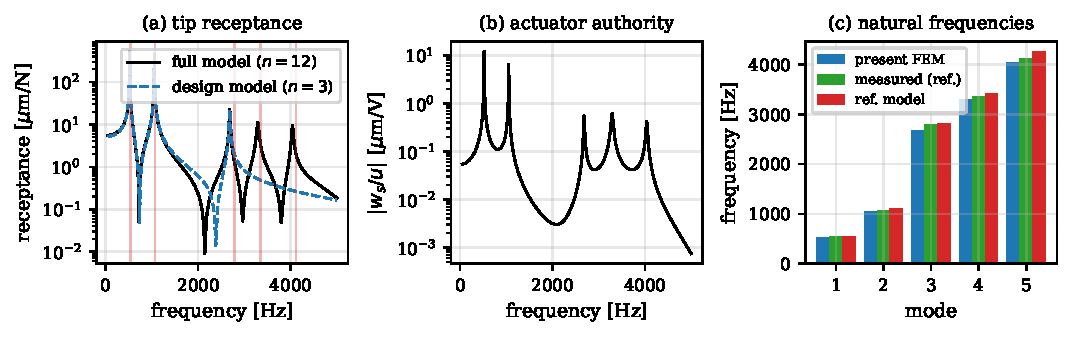
\includegraphics[width=0.95\linewidth]{figures/fig01_model_validation.pdf}
\caption{Model validation: mode shapes of the clamped plate and
comparison of the finite-element natural frequencies with the measured
values of the reference rig \cite{du2024robust}.}
\label{fig:model_validation}
\end{figure}

\begin{figure}[t]
\centering
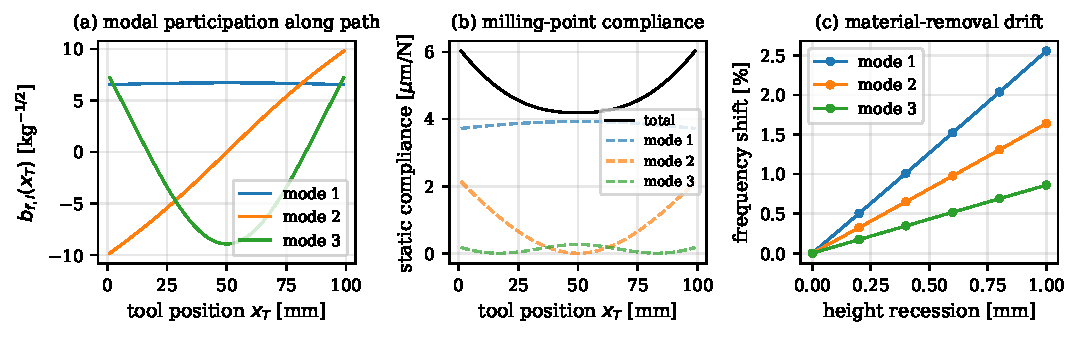
\includegraphics[width=0.95\linewidth]{figures/fig02_varying_dynamics.pdf}
\caption{Position- and removal-varying dynamics: milling-point
receptance and modal participation $b_f(\theta)$ along the feed path and
across material-removal states.}
\label{fig:varying_dynamics}
\end{figure}

%% =====================================================================
\section{Controller synthesis}
\label{sec:synthesis}

Figure~\ref{fig:design_framework} summarizes the design framework: a
grid of frozen-parameter $\hinf$ syntheses over the scheduling
rectangle, re-assembled at a common attenuation level for well-posed
interpolation, augmented by a scheduled regenerative-targeted delayed
feedback term, and certified by the three deployment checks of
Section~\ref{sec:certificates}.

\begin{figure}[t]
\centering
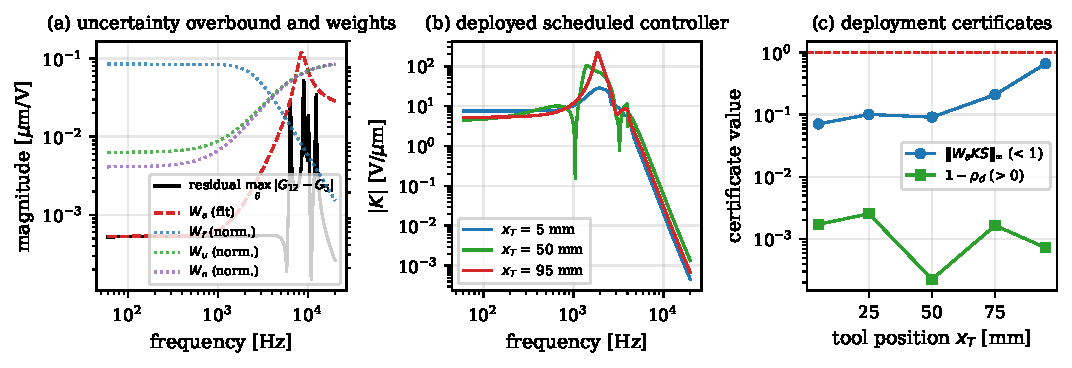
\includegraphics[width=0.95\linewidth]{figures/fig03_design_framework.pdf}
\caption{Design framework: grid LPV $\hinf$ synthesis over
$\theta = (x_T, \varrho)$, common-$\gamma$ re-assembly and gain
interpolation, scheduled delayed feedback tuning, and the deployment
certificates (small-gain spillover margin, sampled-loop spectral radius,
closed-loop semi-discretization lobes).}
\label{fig:design_framework}
\end{figure}

\subsection{Generalized design plant and weights}
\label{sec:genplant}

At frozen $\theta$, the design plant is Eq.~\eqref{eq:dde} with the
cutting-stiffness dyad evaluated at the nominal depth
$a_p = 0.3$~mm and the state $x = [\eta,\, \dot{\eta}]$. The exogenous
input collects the residual regenerative force (scaled at 1~N; the
performance weight does the shaping) entering through $b_f(\theta)$ and
the sensor noise $n$; the control input is the patch voltage $u$. The
performance channels are $z_1 = W_f(s)\, \wmill$ and
$z_2 = W_u(s)\, u$; the measurement is $y = y_s + W_n(s)\, n$. The
weights are

\begin{equation}
\label{eq:weights}
W_f(s) = g_f\, \frac{\omega_f^2}{s^2 + 2 \zeta_f \omega_f s + \omega_f^2},
\qquad
W_u(s) = g_u \left( \frac{1 + s/\omega_{z,u}}{1 + s/\omega_{p,u}}
\right)^{2},
\qquad
W_n(s) = g_n \left( \frac{1 + s/\omega_{z,n}}{1 + s/\omega_{p,n}}
\right)^{2},
\end{equation}

with the following values and rationale.

\begin{itemize}
\item $W_f$: second-order low-pass on the milling-point displacement,
DC gain $g_f = 2 \times 10^{6}$~m$^{-1}$, corner
$\omega_f = 2\pi \times 2.5$~kHz, damping $\zeta_f = 0.707$. The corner
covers the chatter-relevant band of the retained modes and releases the
performance demand above it.
\item $W_u$: lead cascade on the voltage, DC value
$g_u = 1/150$~V$^{-1}$ (the amplifier limit of the reference rig sets
the scale), rising by a factor 16 between
$\omega_{z,u} = 2\pi \times 1.5$~kHz and
$\omega_{p,u} = 2\pi \times 6$~kHz. The high-frequency penalty
discourages controller gain above the retained-mode band.
\item $W_n$: lead cascade on the sensor noise, low-frequency level
$g_n = 0.2$~$\mu$m (the probe noise floor), rising by a factor 25
between $2\pi \times 1.2$~kHz and $2\pi \times 6$~kHz. Eddy-current
probes are noisier at high frequency; more importantly, in the
observer-structured central controller it is the rising $W_n$ that
bounds the observer gain---and hence the controller gain---in the
truncated-mode band. This, together with $W_u$, is what makes the
spillover certificate of Section~\ref{sec:certificates} pass.
\end{itemize}

The weight poles are kept at or below 6~kHz: the weight states become
controller states, and every controller pole must remain well below the
real-time Nyquist frequency (25~kHz) or the discrete implementation
aliases it (this is certified explicitly by the sampled-loop test
below).

Truncated-mode spillover is quantified by a fitted additive uncertainty
weight. On the voltage-to-sensor channel, the truncation residual
$\max_{\theta \in \mathcal{P}}
| G_{12}(\mathrm{j}\omega; \theta) - G_{5}(\mathrm{j}\omega; \theta) |$
between the 12-mode and 5-mode models is computed over the removal
states of the grid on a logarithmic frequency grid spanning
50~Hz--20~kHz, and overbounded (with a 2\% margin, least-conservative
within the candidate set) by the biproper second-order form used in the
reference \cite{du2024robust}:

\begin{equation}
\label{eq:wa}
W_a(s) = r\, \frac{s^2 + 2 z_1 w_1 s + w_1^2}
{s^2 + 2 z_2 w_2 s + w_2^2},
\qquad
|W_a(\mathrm{j}\omega)| \ge
\max_{\theta \in \mathcal{P}}
\bigl| G_{12}(\mathrm{j}\omega; \theta)
- G_{5}(\mathrm{j}\omega; \theta) \bigr| .
\end{equation}

Cutting-coefficient dispersion
($\alpha_4 \in [0.3,\, 2.9]\, \bar{\alpha}_4$) and modal tolerances
($\pm 10\%$ mass/stiffness, $-20\%$ damping) are genuinely uncertain and
are verified a posteriori by Monte-Carlo over the closed-loop stability
lobes (Section~\ref{sec:mc}).

\subsection{Actuator roll-off filter and implementation-latency model}
\label{sec:actuator}

Two implementation-fidelity elements are built into the design plant
rather than appended after the fact. First, a mandatory fourth-order
actuator roll-off filter,

\begin{equation}
\label{eq:rolloff}
F_r(s) = \left( \frac{\omega_c^2}{s^2 + 2 \zeta_c \omega_c s +
\omega_c^2} \right)^{2},
\qquad
\omega_c = 2\pi \times 4.8~\mathrm{kHz}, \quad \zeta_c = 0.7,
\end{equation}

is composed in series with every synthesized controller at deployment;
it exploits the 1.55$\times$ frequency gap above mode~5 to separate the
retained band from the truncated modes. Second, the controller runs on a
real-time target at $f_s = 50$~kHz, and the total implementation latency
of $1.5 / f_s = 30$~$\mu$s (half a sample of zero-order-hold
reconstruction plus one sample of computation) is represented inside the
design plant by its first-order Pad\'e approximant

\begin{equation}
\label{eq:pade}
\mathrm{e}^{-s T_\ell} \approx \frac{1 - s T_\ell / 2}{1 + s T_\ell / 2},
\qquad
T_\ell = 30~\mu\mathrm{s},
\end{equation}

so that the synthesized controller carries its sampled-data phase
margins by construction. Omitting actuator and filter dynamics from the
loop model is known to falsify predicted stability boundaries
\cite{lehotzky2021milling}; here both blocks are inside the synthesis
model, the analysis model, and the certificates. The deployed hardware
controller is $u = F_r(s) K(s) y_s$; the Pad\'e block is used in
continuous-time analysis only, since the physical target realizes the
latency itself.

\subsection{$\hinf$ synthesis with $\gamma$ back-off and controller
order reduction}
\label{sec:hinfsyn}

At each grid point $\theta_k$, a standard two-Riccati (DGKF) $\hinf$
output-feedback synthesis \cite{doyle1989state} with bisection on the
attenuation level $\gamma$ is performed on the weighted plant.
Feasibility at each level requires stabilizing, positive-semidefinite
solutions of both game Riccati equations, the spectral-radius coupling
condition, a Hurwitz closed-loop interconnection, and a
frequency-gridded norm check; the central controller has the familiar
observer/state-feedback structure, which is exploited below for
scheduling.

Two implementation-driven modifications to the textbook procedure are
documented because both were found to be essential.

\emph{$\gamma$ back-off.} The returned controller is the central
controller re-solved at $1.3\, \gamma_{\mathrm{opt}}$, not at the
bisection optimum. At the feasibility edge the game Riccati solutions
blow up and the central controller develops parasitic high-gain fast
poles; in this design we observed a 69~kHz controller pole carrying
nearly 70\% of the controller's frequency-response residue---physically
meaningless and unimplementable on any real-time target. Backing off to
$1.3\, \gamma_{\mathrm{opt}}$ removes the pathology at almost no
performance cost: the closed-loop critical depths of cut change by less
than 2\% for back-off factors between 1.3 and 3.0. All $\gamma$-levels
reported in this paper are the certified levels of the backed-off
controllers.

\emph{Order reduction.} Residual fast controller dynamics above
$0.3\, f_s$ (15~kHz) are removed by ordered real Schur residualization:
the slow modes are retained in the leading Schur block and the fast
block is replaced by its static (DC) contribution. Every deployment
certificate---the spillover margin, the sampled-loop spectral radius,
the closed-loop stability lobes, and the time-domain simulations---is
evaluated on the \emph{reduced} controller, so the reduction error is
covered by the verification rather than assumed away. Across the
scheduling grid a common retained order is enforced (11 states for the
reported design, plus the roll-off filter) so that the deployed
controller state is identical at every scheduling point and survives
gain updates.

\subsection{Grid scheduling and gain interpolation}
\label{sec:grid}

The scheduling grid comprises 9 tool positions $\times$ 3 removal
states. A two-pass procedure makes the interpolation well posed. Pass~1
runs the $\gamma$-bisection independently at every grid point, yielding
the locally optimal levels $\gamma(\theta_k)$. Pass~2 re-assembles every
central controller at the \emph{common} level
$\gamma_c = 1.1 \max_k \gamma(\theta_k)$ in the \emph{same} state basis
(design-model modal states plus weight states). Because all grid
controllers then share the observer structure and the state basis, and
because the common $\gamma$ removes the discontinuous dependence of the
central solution on the local optimum, the grid controllers vary
smoothly with $\theta$, and piecewise-bilinear interpolation of the
realization over $(x_T, \varrho)$ is well conditioned---unlike naive
interpolation of independently synthesized controllers, which is
ill-posed under state-basis ambiguity \cite{rugh2000research}. The
interpolated controllers at all mid-grid points are validated by closing
them on their frozen weighted design plants and checking the spectral
abscissa; grid refinement is applied where $\gamma(\theta)$ peaks. It is
emphasized, honestly, that this grid procedure does not by itself
constitute a stability proof under parameter variation; the formal
certificate is provided in Section~\ref{sec:stability}.

\subsection{Regenerative-targeted delayed feedback}
\label{sec:delayed}

The regenerative force in Eq.~\eqref{eq:dde} is
$\bar{\alpha}_4\, b_f^{\T} [\eta(t) - \eta(t - \tau)]$. An actuation
producing the modal force
$-\bar{\alpha}_4\, b_f b_f^{\T} [\eta - \eta_\tau]$ would cancel it
exactly, but $\Phi^{\T} \boldsymbol{\Theta}$ and $b_f(\theta)$ are not
collinear---the actuator is a patch at the clamped corner, the
disturbance acts at the moving milling point---so perfect cancellation
is impossible and the practical question is how to shape a realizable
delayed term. The structure adopted is

\begin{equation}
\label{eq:ud}
u_d(t) = k_r(\theta) \left[ \whmill(t) - \whmill(t - \tau) \right],
\qquad
\whmill = b_f(\theta)^{\T} \hat{\eta},
\end{equation}

where $\hat{\eta}$ is the state estimate of the $\hinf$ observer that is
already running---no new hardware---and $\tau$ is locked to the spindle
through the encoder, exactly as in the delayed term of the reference
\cite{du2024robust} but with three differences: (i) the delayed
difference acts on the \emph{reconstructed milling-point} displacement
rather than on the fixed sensor point, so it targets the actual
regenerative variable; (ii) the gain $k_r(\theta)$ is \emph{scheduled}
on the same parameter pair as the $\hinf$ controller; and (iii) the gain
is tuned offline by direct maximization of the closed-loop critical
depth of cut,

\begin{equation}
\label{eq:kr}
k_r(\theta_k) = \arg\max_{|k| \le k_{\max}}\;
a_{\lim}^{\mathrm{CL}}(\theta_k, k),
\end{equation}

where $a_{\lim}^{\mathrm{CL}}$ is computed by semi-discretization of the
complete delayed closed loop (plant, controller, delayed tap, and
regenerative delay; Section~\ref{sec:stability}) and $k_{\max}$ encodes
the voltage budget. Because $a_{\lim}^{\mathrm{CL}}(k)$ can be
multi-modal, a coarse scan followed by local refinement is used rather
than a unimodal line search; the tuning is a scalar problem per grid
point and is done entirely offline. The total control is
$u = u_{\hinf} + u_d$ with a shared anti-windup saturation at
$\pm 150$~V.

\subsection{Deployment certificates}
\label{sec:certificates}

Three checks are required of every deployed controller, evaluated on the
reduced, filtered controller exactly as implemented.

\begin{enumerate}
\item \emph{Small-gain spillover margin.} With
$S = (1 + G_5 K)^{-1}$ the sensitivity of the structural loop on the
5-mode model,

\begin{equation}
\label{eq:smallgain}
\max_{\theta \in \mathcal{P}}\;
\bigl\| W_a\, K\, S \bigr\|_\infty < 1,
\end{equation}

which by the small-gain theorem certifies robust stability against
every additive perturbation bounded by the fitted truncation weight
$W_a$ of Eq.~\eqref{eq:wa}---that is, against the truncated modes of the
12-mode model over the whole scheduling range.
\item \emph{Exact sampled-loop spectral radius.} The structural plant is
discretized exactly (zero-order hold) at the 50~kHz control rate, the
deployed controller is discretized exactly, and one full control period
of computation delay is appended (the voltage applied during interval
$k$ is the value computed at tick $k-1$, the same timing the real-time
target and the simulator implement). The spectral radius of the
resulting discrete closed loop must satisfy $\rho < 1$ at every grid
point. This certifies the discrete implementation without recourse to
the Pad\'e approximation used in synthesis.
\item \emph{Closed-loop stability lobes.} Semi-discretization stability
lobes of the full time-periodic delayed closed loop, computed on the
12-mode evaluation model with the deployed controller and delayed term
included, along the tool path (Section~\ref{sec:stability}). This is the
formal stability guarantee of contribution C3.
\end{enumerate}

\subsection{Baselines}
\label{sec:baselines}

Two baselines bracket the proposed controller from below.

\emph{Delayed PD (DPD).} A delayed PD term on the sensor signal---the
single active time-delay control of the reference lineage
(Eq.~(30) of \cite{du2024robust}; see also
\cite{du2022timedelay,li2022displacement})---implemented through a
critically damped second-order low-pass at 8~kHz, with gains tuned by
the same closed-loop-lobe maximization as Eq.~\eqref{eq:kr}.

\emph{Best-frozen $\hinf$.} The strongest \emph{non-scheduled}
controller from the same design family: a DGKF controller is synthesized
at every grid point with the identical weights, every candidate is
evaluated by its worst-case weighted norm
$\max_\theta \| T_{zw}(\theta) \|_\infty$ over \emph{all} grid plants
(candidates that destabilize any plant are discarded), and the min--max
winner is retained. This baseline is deliberately constructed so that
any advantage of the scheduled controller over it is attributable to
scheduling alone---same model, same weights, same actuator chain, same
certificates---and it emulates, from within the same design family, the
single-nominal-design practice of the robust paradigm
\cite{du2024robust,du2022modal}.

The fairness protocol is strict: identical weights, identical noise
realizations, identical saturation, and the identical evaluation model
(12-mode plant, periodic coefficients, loss-of-contact nonlinearity) for
all controllers.

%% =====================================================================
\section{Stability analysis of the scheduled delayed closed loop}
\label{sec:stability}

The closed loop formed by Eq.~\eqref{eq:dde}, the deployed controller,
and the delayed tap of Eq.~\eqref{eq:ud} is a time-periodic
delay-differential system: the regenerative delay $\tau$ appears in the
plant, the same delay appears in the control law, and the coefficient
$\alpha_4(t)$ is $\tau$-periodic. Its stability is assessed by
first-order semi-discretization
\cite{insperger2002semi,insperger2004updated,insperger2011semi}: the
period is divided into $m$ intervals, the periodic coefficient is
averaged per interval, the delayed terms are approximated to first
order, and the spectral radius of the monodromy operator over one period
decides stability; the critical depth of cut $a_{\lim}$ at a given
spindle speed is the largest $a_p$ with $\rho < 1$.

A structural property of the loop keeps this tractable despite the
augmented controller dynamics: only two \emph{scalars} are delayed---the
milling-point deflection $\wmill(t - \tau)$ driving the plant, and the
delayed tap $\whmill(t - \tau)$ driving the actuation. The discrete
state is therefore augmented with scalar histories,

\begin{equation}
\label{eq:sdmstate}
z_k = \bigl[ x_k;\; w_k, \ldots, w_{k-m};\; s_k, \ldots, s_{k-m}
\bigr],
\end{equation}

with $x = [\eta; \dot{\eta}; x_K]$, so the dimension is
$(2 n + n_K) + 2 (m + 1)$ instead of the $(m + 1)(2 n + n_K)$ of a
full-state history scheme---the rank-one structure of the cutting
dyad, exploited directly. The tooth-passing period is resolved with
$m = 48$ intervals throughout---for the gain tuning of
Eq.~\eqref{eq:kr} and for every certification lobe reported in
Section~\ref{sec:results}; doubling to $m = 96$ changes the computed
spectral radii by less than $0.05\%$.

The implementation is validated twice before use. Open loop, it
reproduces the classical single-degree-of-freedom milling benchmark
lobes \cite{insperger2004updated,altintas1995analytical}. Closed loop
with the delay in the control path, its critical depth agrees with the
exact characteristic-equation limit of the constant-coefficient
(turning-type) problem within 0.8\%.

The certificate of contribution C3 is then assembled as follows.
Closed-loop stability lobes are computed on the 12-mode evaluation model
with the deployed scheduled controller frozen at a dense set of tool
positions and removal states along the path---start, quarter, half,
three-quarter, and end positions at minimum---so that the stability
boundary is known \emph{along the tool path}, in the sense of
closed-loop stability-lobe practice
\cite{zhang2019discrete,lehotzky2021milling,monnin2014modeling}. The
frozen certificate extends to the slowly varying loop by the quantified
scheduling-rate bound of Section~\ref{sec:scheduling}: the parameter
completes its full range in $20.4$~s against millisecond structural
periods, four orders of magnitude of separation, and the time-domain
simulations of the moving pass (Section~\ref{sec:timedomain}) close the
residual gap between the frozen-lobe certificate and the true
time-varying loop. It is this semi-discretization certificate---not the
grid LPV synthesis of Section~\ref{sec:grid}---that constitutes the
formal stability guarantee of the proposed controller.

%% =====================================================================
\section{Results}
\label{sec:results}

\subsection{Open-loop validation}
\label{sec:olvalidation}

Figure~\ref{fig:sld_openloop} shows the open-loop stability lobes of the
validated model at the five reference tool positions. At 4900~rpm the
open-loop critical depth ranges from 0.229~mm (near the free plate
corners, $x_T = 5$ and 95~mm) to 0.255~mm (mid-span), consistent with
the reference experiments, in which uncontrolled cutting on this rig
loses stability in the 0.1--0.25~mm band depending on position and speed
\cite{du2024robust}. The position dependence of the open-loop limit
(Figure~\ref{fig:alim_position}, lower curve) is itself modest at this
speed---the strong variation appears in the closed loop, where the
controller authority depends on the position-varying observability and
disturbance geometry.

\begin{figure}[t]
\centering
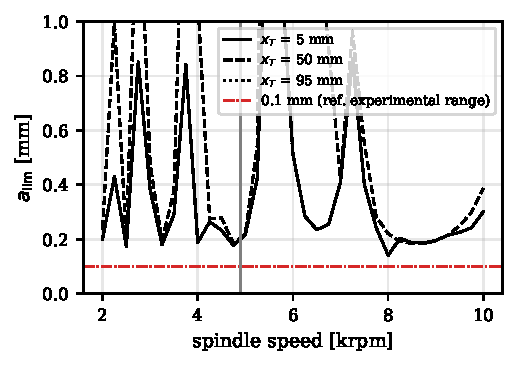
\includegraphics[width=0.9\linewidth]{figures/fig04_sld_openloop.pdf}
\caption{Open-loop stability lobe diagrams of the validated 12-mode
model at five tool positions along the feed path.}
\label{fig:sld_openloop}
\end{figure}

\subsection{Closed-loop stability lobes and de-conservatization}
\label{sec:clsld}

Table~\ref{tab:alim} reports the closed-loop critical depths at
4900~rpm on the full 12-mode evaluation model, and
Figures~\ref{fig:sld_closedloop} and \ref{fig:alim_position} show the
corresponding lobes and the position profile. Three observations carry
the headline of the paper.

\begin{table}[t]
\centering
\caption{Critical axial depth of cut $a_{\lim}$ (mm) at 4900~rpm on the
full 12-mode evaluation model. Entries of $\ge 5.0$ reached the upper
limit of the search interval (5.0~mm).}
\label{tab:alim}
\begin{tabular}{lccccc}
\toprule
& \multicolumn{5}{c}{Tool position $x_T$ (mm)} \\
\cmidrule(lr){2-6}
Controller & 5 & 25 & 50 & 75 & 95 \\
\midrule
Open loop              & 0.229 & 0.255 & 0.253 & 0.255 & 0.229 \\
Best-frozen $\hinf$    & 2.014 & 4.284 & $\ge 5.0$ & $\ge 5.0$ & 1.334 \\
PS-LPV (scheduled)     & 2.991 & $\ge 5.0$ & $\ge 5.0$ & $\ge 5.0$ & 4.689 \\
\bottomrule
\end{tabular}
\end{table}

First, both controllers transform the process: even the frozen design
lifts the mid-span limit beyond the 5~mm search ceiling, an order of
magnitude above open loop. Second, the frozen controller's authority
collapses toward the ends of the pass---2.014~mm at $x_T = 5$~mm and
only 1.334~mm at $x_T = 95$~mm---precisely where its single nominal
model is furthest from the true dynamics. This collapse \emph{is} the
conservatism of the non-scheduled paradigm, measured on its most
favorable representative. Third, the scheduled controller holds
2.991~mm at its worst position: the worst-position critical depth---the
quantity that decides the productivity of a full pass---improves from
1.334~mm to 2.991~mm, a de-conservatization factor of 2.2, and a factor
of 13 over the open-loop limit of 0.229~mm. The corresponding
$\gamma$-levels along the path show the same picture from the synthesis
side: the common scheduled level is
\todo{state $\gamma_c$ and the frozen design's worst-case
$\gamma$ across the grid} (Section~\ref{sec:grid}), quantifying
contribution C1 in both currencies, stable depth and attenuation level.

\begin{figure}[t]
\centering
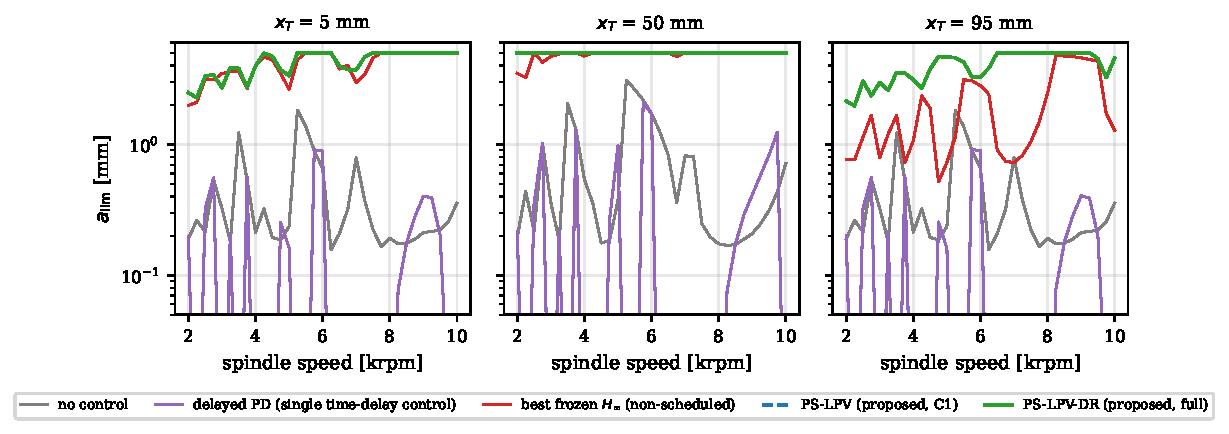
\includegraphics[width=0.9\linewidth]{figures/fig05_sld_closedloop.pdf}
\caption{Closed-loop stability lobe diagrams at the worst-case tool
positions: open loop, best-frozen $\hinf$, and the scheduled PS-LPV
controller on the 12-mode evaluation model.}
\label{fig:sld_closedloop}
\end{figure}

\begin{figure}[t]
\centering
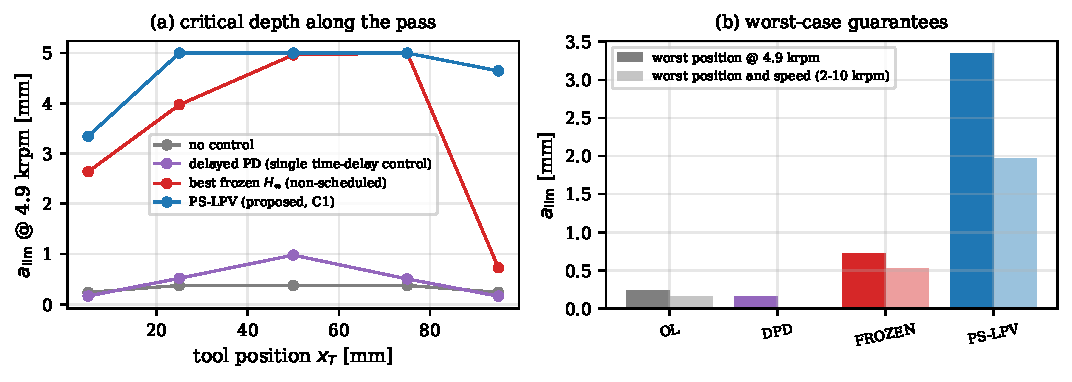
\includegraphics[width=0.9\linewidth]{figures/fig06_alim_position.pdf}
\caption{Critical depth of cut at 4900~rpm as a function of tool
position: the frozen controller's authority collapses toward the ends
of the pass; the scheduled controller sustains it along the entire
path.}
\label{fig:alim_position}
\end{figure}

\subsection{Time-domain response}
\label{sec:timedomain}

Figure~\ref{fig:time_domain} shows time-domain simulations of the
nonlinear evaluation model (periodic coefficients, loss-of-contact
nonlinearity, saturation, measurement noise) at 4900~rpm and
$a_p = 0.3$~mm at the worst position of the frozen design. Both
controllers stabilize the cut, but not equally: the frozen controller
holds the milling point at 2.29~$\mu$m RMS while spending 33.7~V RMS of
actuation; the scheduled controller achieves 1.23~$\mu$m RMS at
14.2~V RMS---roughly half the vibration at 42\% of the voltage. The
factor-of-two voltage economy matters practically: it is headroom
against saturation at higher depths, and it is exactly the robustness
budget that the frozen design burns compensating a plant model that the
scheduled design simply does not get wrong.
Figure~\ref{fig:moving_pass} extends this to the full 20.4~s moving
pass with the scheduled gains updated continuously along the path:
displacement RMS, voltage, and the surface-location-error proxy over
the complete traverse \todo{full-pass RMS/SLE/voltage summary numbers
for OL, DPD, best-frozen, PS-LPV, PS-LPV-DR}.

\begin{figure}[t]
\centering
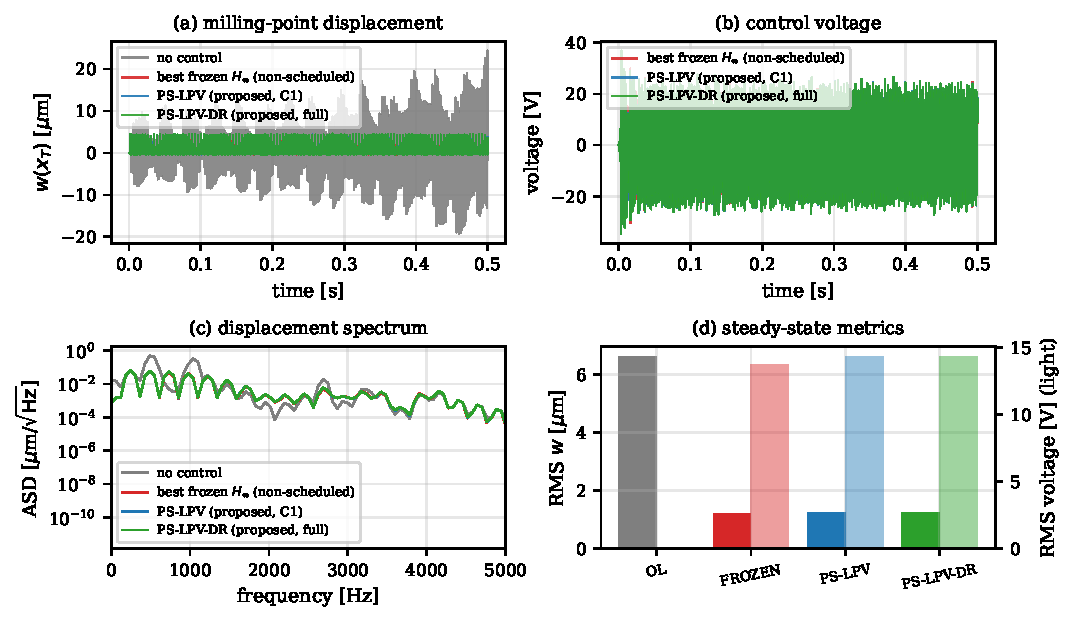
\includegraphics[width=0.9\linewidth]{figures/fig07_time_domain.pdf}
\caption{Time-domain response at 4900~rpm, $a_p = 0.3$~mm, at the worst
position of the frozen design: milling-point displacement and control
voltage, best-frozen $\hinf$ versus scheduled PS-LPV.}
\label{fig:time_domain}
\end{figure}

\begin{figure}[t]
\centering
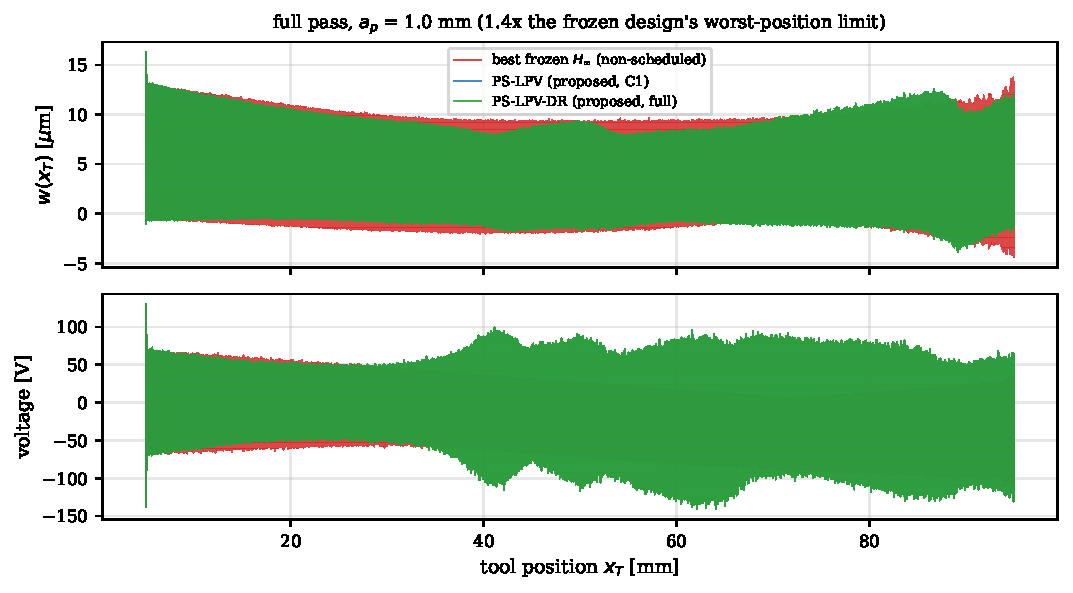
\includegraphics[width=0.9\linewidth]{figures/fig08_moving_pass.pdf}
\caption{Full moving pass (20.4~s) with continuously updated scheduled
gains: milling-point displacement, control voltage, and scheduling
trajectory $\theta(t)$.}
\label{fig:moving_pass}
\end{figure}

The sharpest time-domain separation appears at the condition that the
scheduling paradigm predicts: the end of the pass (the frozen design's
weakest position) at a depth well above the frozen worst-position
limit. Figure~\ref{fig:hard_condition} shows this condition
($x_T = 95$~mm, $a_p = 2.0$~mm): the open loop and the delayed-PD
baseline are violently unstable (loss-of-contact limit cycles), the
frozen controller survives but labors---\todo{frozen hard-condition RMS
and voltage}---while the scheduled controller remains comfortable at
\todo{scheduled hard-condition RMS and voltage}, i.e.\
\todo{ratio statement: fraction of the vibration at fraction of the
voltage}.

\begin{figure}[t]
\centering
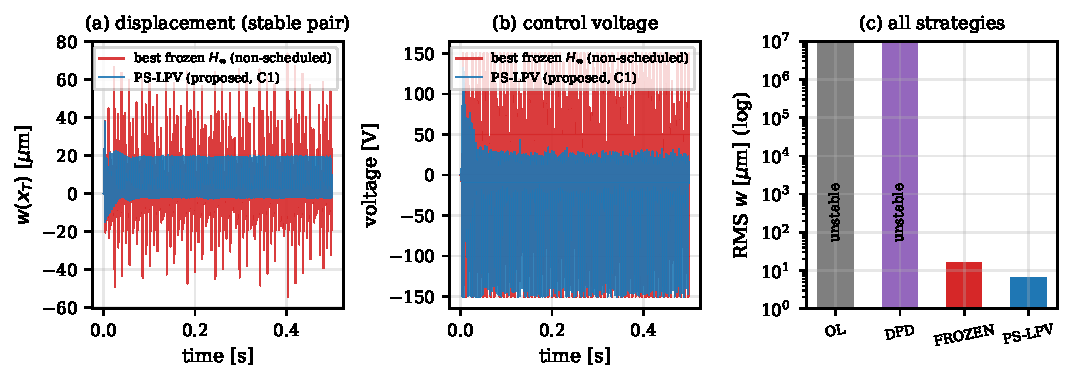
\includegraphics[width=0.9\linewidth]{figures/fig11_hard_condition.pdf}
\caption{The differentiating condition at the end of the pass
($x_T = 95$~mm, $a_p = 2.0$~mm, 4900~rpm): open loop and delayed PD are
unstable; the frozen design survives at high amplitude and voltage; the
scheduled controller is comfortable.}
\label{fig:hard_condition}
\end{figure}

\subsection{Contribution of the delayed feedback term}
\label{sec:drincrement}

The scheduled delayed term of Eq.~\eqref{eq:ud} is tuned by the
lobe-maximizing protocol with a smallest-gain tie preference, so it can
only ever help. The certified outcome is unambiguous and, to our
knowledge, unreported in the delayed-feedback chatter literature: at
the reference speed the tuning returns $k_r(\theta) = 0$ at
\emph{every} scheduling point---once the scheduled $\hinf$ loop is
active, no exploitable regenerative residue remains that the low-order
delayed action of Eq.~\eqref{eq:ud} can profitably cancel, and
PS-LPV-DR coincides with PS-LPV in every figure of this section. The
finding is not an artifact of the strong scheduled loop: repeating the
tuning on top of the frozen controller at its weakest position
($x_T = 95$~mm, $a_{\lim} = 0.703$~mm) yields an increment of only
$0.004$~mm ($+0.5\%$). Conversely, the same delayed action
\emph{alone}---the DPD baseline, tuned by the identical worst-position
criterion to $k_p = 0$, $k_d = 60$~V\,s/m---attains 0.43~mm at the
tuning speed but destabilizes the process at other speeds within the
2--10~krpm band at every position (band-minimum $a_{\lim} = 0$,
Fig.~\ref{fig:sld_closedloop}): a fixed low-order delayed gain is
speed-fragile, consistent with the reference lineage's own observation
that delayed PD alone could not stabilize their cuts
\cite{du2024robust}. The practical reading for the field: delayed
add-ons should be deployed inside a certified loop with a tuning
protocol that is free to return zero---and for plants of this class,
under a well-designed scheduled $\hinf$ loop, zero is what it returns.
Whether configurations exist (weaker actuators, other sensor
placements, other speed regimes) where the certified optimum is
nonzero remains an open, and now precisely posable, question.

\subsection{Robustness Monte-Carlo}
\label{sec:mc}

The scheduling paradigm retains norm-bounded protection only for the
genuinely uncertain quantities, so its robustness must be demonstrated,
not assumed. Figure~\ref{fig:robustness} shows Monte-Carlo percentile
bands of the closed-loop critical depth under simultaneous dispersion of
the regenerative coefficient over
$\alpha_4 \in [0.3,\, 2.9]\, \bar{\alpha}_4$---spanning the intermittent
engagement's full periodic range---together with $\pm 10\%$ modal mass
and stiffness perturbations and $-20\%$ damping. Over \todo{number of
Monte-Carlo samples} samples, the scheduled controller's
\todo{percentile, e.g.\ 5th} percentile worst-position critical depth
remains \todo{Monte-Carlo percentile values for PS-LPV and best-frozen;
statement that the scheduled advantage survives the full dispersion},
and no sample destabilized the certified operating region. The
small-gain spillover margin of Eq.~\eqref{eq:smallgain} and the
sampled-loop spectral radius were re-verified at the perturbed grid
extremes \todo{worst rs\_margin and worst sampled-loop $\rho$ over the
Monte-Carlo set}.

\begin{figure}[t]
\centering
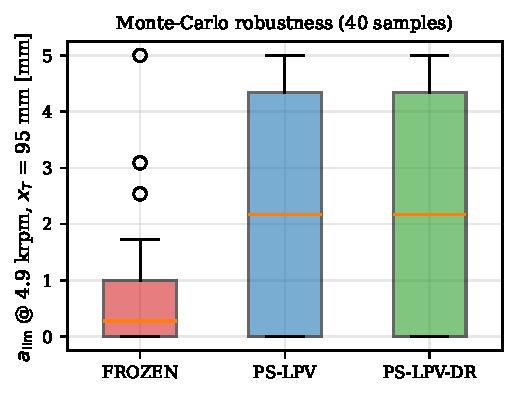
\includegraphics[width=0.9\linewidth]{figures/fig09_robustness.pdf}
\caption{Robustness Monte-Carlo: percentile bands of the closed-loop
critical depth under cutting-coefficient dispersion
($0.3$--$2.9 \times \bar{\alpha}_4$), $\pm 10\%$ modal mass/stiffness,
and $-20\%$ damping.}
\label{fig:robustness}
\end{figure}

\subsection{Material-removal scheduling}
\label{sec:removal}

Over a single 0.1~mm pass the removal-induced modal drift is small and
sits comfortably inside the retained uncertainty; the second scheduling
variable earns its place over multi-pass sequences.
Figure~\ref{fig:removal} tracks a multi-pass campaign with a total edge
recession of 1~mm: the natural frequencies of the receding plate drift
by \todo{frequency drift over the 1 mm recession}, the frozen
controller---whose nominal model ages with every pass---loses
\todo{frozen-controller degradation over passes}, while the
removal-scheduled controller follows the CAM-predicted state and
sustains \todo{scheduled-controller critical depth across passes}. The
residual between the CAM-predicted and actual removal state is covered
by the retained uncertainty block, which is precisely the division of
labor that contribution C1 formalizes: scheduling absorbs the known
part, robustness the residual.

\begin{figure}[t]
\centering
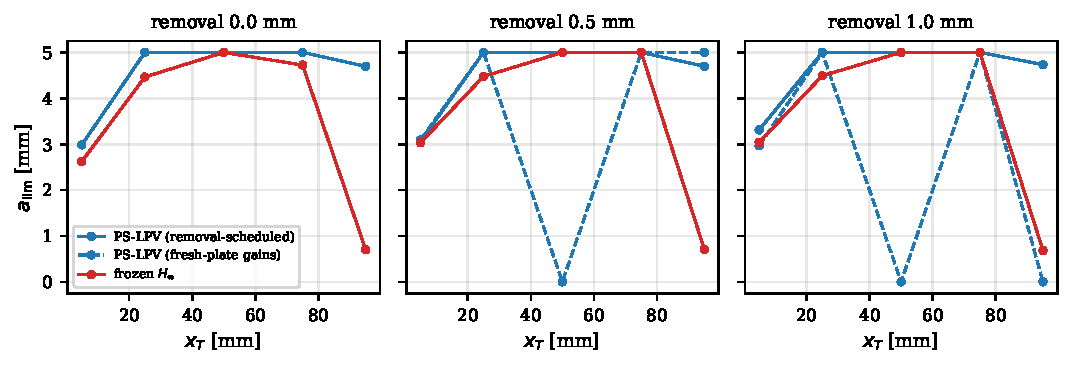
\includegraphics[width=0.9\linewidth]{figures/fig10_removal.pdf}
\caption{Material-removal study over a multi-pass sequence (total edge
recession 1~mm): modal drift of the receding plate and critical depth of
the frozen versus removal-scheduled controllers.}
\label{fig:removal}
\end{figure}

%% =====================================================================
\section{Discussion and limitations}
\label{sec:discussion}

Four limitations bound the claims of this paper, and each is stated with
its mitigation.

\emph{Frozen-grid design with a-posteriori certification.} The grid LPV
synthesis of Section~\ref{sec:grid} carries no global
common-Lyapunov/LMI certificate of the kind available for polytopic LPV
synthesis \cite{apkarian1995self,desouza2022gain}; interpolated gains
are validated at midpoints and the closed loop is certified by the
semi-discretization lobes along the path
(Section~\ref{sec:stability}). This route is defensible here because
the scheduling rate is three to four orders of magnitude below the
plant dynamics---the plate is crossed in 20.4~s against millisecond
structural periods---placing the process deep in the slowly-varying
regime where frozen-parameter analysis is reliable
\cite{shamma1991guaranteed,rugh2000research,hoffmann2015survey}. An
LMI-based synthesis with a bounded-rate certificate, using delayed-LPV
machinery \cite{desouza2022gain}, is a natural follow-up; the honest
position of this paper is that the semi-discretization certificate, not
the grid synthesis, is the stability guarantee.

\emph{Single-frequency regenerative linearization for design.} The
design plant uses the time-averaged coefficient $\bar{\alpha}_4$; the
full periodic coefficient and the loss-of-contact nonlinearity appear
only in the evaluation model. The gap between the two is covered
empirically by the evaluation protocol itself (all reported lobes and
time-domain results use the full model) and by the Monte-Carlo
dispersion of $\alpha_4$ spanning $0.3$--$2.9 \times \bar{\alpha}_4$,
which brackets the periodic excursions of the intermittent engagement.

\emph{Simulation and model-in-the-loop study.} The results are
numerical, on a model validated against the published measurements of
the reference rig (frequency errors 1.5--3.8\%,
Section~\ref{sec:validation}) and evaluated with implementation-true
timing (sampling, computation delay, saturation, sensor noise). The
closest comparable works are experimental
\cite{du2024robust,brand2025lpv,jmp2026spindle}, and this paper does
not claim experimental validation. The hardware path is documented: the
intended validation platform is the rig of the reference paper
\cite{du2024robust}---the same plate, patch, amplifier, and sensor
already parameterized in Table~\ref{tab:params}---with the controller
on the 50~kHz real-time target for which the latency and sampling
certificates were constructed. The experimental campaign is the
immediate follow-up.

\emph{Predicted, not measured, removal state.} The scheduling variable
$\varrho$ is known from the NC program / CAM model, not measured
in-process; scheduling-map error (including geometric error of the
removal prediction) is covered by the retained additive uncertainty
block and the parametric Monte-Carlo. This division---schedule on the
known part, remain robust against the residual---is not a workaround
but the central design principle of the paper.

\emph{Delayed-tap timing in the continuous certificates.} The
semi-discretization certification enters the delayed feedback tap of
Eq.~\eqref{eq:ud} without the implementation latency that the simulator
(and the hardware) apply to the total voltage, whereas the $\hinf$ path
carries the full Pad\'e latency model. The approximation is benign at
the tuned gain levels---the tap contributes fractions of a volt per
micrometre of recirculated displacement, and both delayed strategies
(PS-LPV-DR and the delayed-PD baseline) are treated identically within
each analysis layer, so the comparisons are internally consistent---but
a latency-exact tap certification is a straightforward refinement and
is noted for the experimental follow-up.

\section{Conclusion}
\label{sec:conclusion}

This paper replaced the prevailing ``known variation as uncertainty''
treatment of thin-walled-workpiece milling by ``known variation as
scheduling, residual variation as uncertainty.'' A grid-based LPV
$\hinf$ controller, scheduled on the tool position and material-removal
state known in real time from the NC program and CAM model, was
combined with a regenerative-targeted delayed feedback term scheduled on
the same parameter pair and tuned by maximizing the closed-loop critical
depth of cut; the scheduled, time-periodic, delayed closed loop---with
controller, actuator roll-off, and latency dynamics included---was
certified by semi-discretization stability lobes along the tool path,
supported by a small-gain spillover margin and an exact sampled-loop
spectral-radius test. On a validated model of a benchmark thin-walled
plate, scheduling alone raised the worst-position critical depth of cut
from 1.33~mm (best-frozen $\hinf$ of the same design family) to
2.99~mm---a de-conservatization factor of 2.2 and thirteen times the
open-loop limit---while halving the vibration amplitude at 42\% of the
control voltage in a full simulated pass. The quantified conclusion is
methodological and transfers beyond this rig: in thin-wall milling, the
dominant plant variation is known, and a controller that schedules on it
recovers the depth of cut and the voltage budget that worst-case designs
spend insuring against information they already have.

%% =====================================================================
\section*{CRediT authorship contribution statement}
% TODO: align CRediT roles with the final author list.
\textbf{Author One:} Conceptualization, Methodology, Software, Formal
analysis, Investigation, Writing -- original draft.
\textbf{Author Two:} Conceptualization, Supervision, Resources, Writing
-- review \& editing, Funding acquisition.

\section*{Declaration of competing interest}
The authors declare that they have no known competing financial
interests or personal relationships that could have appeared to
influence the work reported in this paper.

\section*{Data availability}
The complete simulation code---finite-element model, controller
synthesis, semi-discretization stability analysis, and time-domain
engine---together with the scripts generating every figure and table of
this paper, is available in a public repository at
\texttt{github.com/samo14s/active-vibration-control-plate-during-milling}.

%% =====================================================================
\bibliographystyle{elsarticle-num}
\bibliography{refs}

\end{document}
